
\documentclass[tikz,border=5pt]{standalone}

% Core packages
\usepackage{amsmath,amssymb}
\usepackage{tikz}
\usepackage{tikz-cd}
\usepackage{pgfplots}
\usepackage{multicol}
\usepackage{xcolor}
\usepackage{caption}
\usepackage{float}
\usepackage{kotex}

% TikZ / PGF configuration
\usetikzlibrary{
  arrows.meta,
  calc,
  positioning,
  shapes.geometric,
  shapes.symbols,
  fit,
  backgrounds,
  patterns,
  matrix,
  intersections,
  decorations.pathmorphing,
  decorations.markings,
  angles,
  quotes
}
\pgfplotsset{compat=1.18}

% Reusable TikZ styles
\tikzset{
  >=stealth,
  line cap=round,
  line join=round,
  every picture/.style={line width=0.9pt},
  box/.style={draw, rounded corners, minimum width=2.8cm, minimum height=1.2cm, align=center},
  circlebox/.style={draw, circle, minimum size=1cm, align=center},
  arrow/.style={->, thick},
  dashedarrow/.style={->, thick, dashed},
  point/.style={circle, fill, inner sep=1.2pt},
  gridhelp/.style={help lines, gray!35},
  highlight/.style={fill=blue!10, draw=blue!60!black},
  3D/.style={
    x={(-0.60cm,-0.42cm)},
    y={(0.78cm,0cm)},
    z={(0cm,0.78cm)}
  }
}


\begin{document}

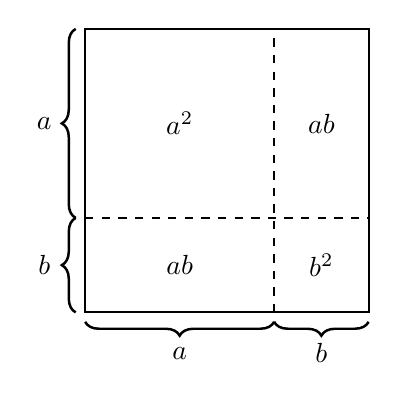
\begin{tikzpicture}[scale=1.2]
    % 전체 사각형 외곽
    \draw[thick] (0,0) rectangle (3,3);
    
    % 내부 분할선
    \draw[dashed] (2,0) -- (2,3);
    \draw[dashed] (0,1) -- (3,1);
    
    % 각 영역의 넓이 표시
    \node at (1,2) {$a^2$};
    \node at (2.5,2) {$ab$};
    \node at (1,0.5) {$ab$};
    \node at (2.5,0.5) {$b^2$};
    
    % 변의 길이 표시
    \draw [decorate,decoration={brace,amplitude=5pt,mirror}] (0,-0.1) -- (2,-0.1) node [black,midway,yshift=-0.4cm] {$a$};
    \draw [decorate,decoration={brace,amplitude=5pt,mirror}] (2,-0.1) -- (3,-0.1) node [black,midway,yshift=-0.4cm] {$b$};
    \draw [decorate,decoration={brace,amplitude=5pt}] (-0.1,1) -- (-0.1,3) node [black,midway,xshift=-0.4cm] {$a$};
    \draw [decorate,decoration={brace,amplitude=5pt}] (-0.1,0) -- (-0.1,1) node [black,midway,xshift=-0.4cm] {$b$};
\end{tikzpicture}

\end{document}

